\documentclass[12pt]{article}

\usepackage{fullpage}
\usepackage{epsfig}
\usepackage{graphicx}

\newcommand{\code}[1]{\texttt{#1}}

\newcommand{\keyword}[1]{\textit{#1}}

\author{Marc G. Bellemare}
\title{Extending the RLAI Robotic Simulator}

\begin{document}

\maketitle

This document is not yet complete. You should probably not rely on it.

\section{Purpose of This Tutorial}

The purpose of this tutorial is to describe how to extend the RLAI Robotic
Simulator. In particular, it details:

\begin{itemize}
\item{How to create new environment descriptions}
\item{How to create new Simulator components}
\end{itemize}

It does not, however, discuss how to use the Simulator or how to create agents.
For this, you may want to refer to the other tutorials, available from the
same location as this tutorial.


\section{High-Level Description of the Simulator Mechanics}

\subsection{Operation and components}

The Simulator core is its \keyword{engine} (class: \code{SimulatorEngine}). 
The Simulator operates at a set 
frequency (by default, 100 time steps per second). On each time step, the
engine updates the world to correspond to the next step. This update is done
by calling the \code{apply()} method of each \keyword{component} 
(class: \code{SimulatorComponent}). in turn. A component 
is a module of the simulator responsible for a specific task. A brief list
of components (and their corresponding class) includes:

\begin{itemize}
  \item{Dynamics: \code{SimulatorComponentDynamics}}
  \item{Visible light: \code{SimulatorComponentLight}}
  \item{Gyroscope: \code{SimulatorComponentGyroscope}}
  \item{...}
\end{itemize}

The \code{apply} method of each component is the core of the Simulator's
computation.

\subsection{Objects}

Aside from a few exceptions, everything that exists in the simulator is an
\keyword{object} (class: \code{SimulatorObject}). An object has a position,
a direction, a label and (possibly) a shape (as a \code{Polygon}). Most 
importantly, each object has a list of properties (states, class 
\code{ObjectState}). An object may also have children to form complex objects
from parts. For example, the simulated Critterbot is composed of a main body
to which are attached sensor objects.

\subsection{Object properties: ObjectState}

The specific nature of an object depends on its properties. In general, each
component acts on one or two properties of an object. For example, the 
component \code{SimulatorComponentDynamics} acts upon 
\code{ObjectStateDynamics} and \code{SimulatorComponentLight} acts upon
\code{ObjectStateLightSource} and \code{ObjectStateLightSensor}. The general
contract of an ObjectState is to provide member variables for its associated
component. \code{ObjectStateLightSource} provides light source-related 
variables corresponding to the object to which it is attached.


With the above tools in hand - objects, components and object states - we
can now consider extending the computational aspects of the Simulator.

\section{Creating new components}

For this section, we will study the Critterbot gyroscope and its associated
component as a running example.

\subsection{Creating ObjectStateGyroscope}

\code{ObjectStateGyroscope} contains various variables and methods of interest.
In this case, gyroscope-related state information only includes the actual 
gyroscope reading (\code{aVelocity}). There is also a variable for the 
relative error of the gyroscope.

\code{ObjectStateGyroscope} implements the following methods inherited from 
\code{ObjectState}:

\begin{enumerate}
  \item{\code{getName()}. Returns a unique identifier for this ObjectState.}
  \item{\code{clone()}. Creates a copy of this ObjectState.}
  \item{\code{draw()}. This method handles drawing additional state information;
    for example, the bump sensors may be displayed as shrinking red circles
    using this method.}
  \item{\code{clearTransient()}. If this `ObjectState' uses any intermediate
    data structures during the computation of its value, this mehtod should 
    re-initialize them.}
\end{enumerate}

\code{getName} is usually implemented by returning a static key. This is used
to retrieve the corresponding ObjectState in an object.  Here, we return
\code{ObjectStateGyroscope.NAME}.

\code{clone} creates a new \code{ObjectStateGyroscope} and uses the
\code{copyFrom} method to ensure a deep clone.
\code{draw} is left empty - we do not display any gyroscope information.
\code{clearTransient} sets the reported velocity to 0.


\subsection{Creating SimulatorComponentGyroscope}

\code{SimulatorComponentGyroscope} contains methods that compute gyroscope
state information (stored in \code{ObjectStateGyroscope}), possibly based
on other state information. In this case, the gyroscope readings depend on
the robot's rotational velocity, which we will obtain from 
\code{ObjectStateDynamics}.

\code{SimulatorComponentGyroscope} implements a single method inherited from
\code{SimulatorComponent}: \code{apply()}. The apply method is the simulator's
computational core. Recall that it is called at every iteration of the 
simulator (e.g. every 100th of a second). The apply method takes three 
parameters: two \code{SimulatorState} objects and an integer \code{delta},
the number of milliseconds that we are requesting the system to simulate
(10 by default).

The first \code{SimulatorState} encapsulates the current time step information,
and (by convention) should not be modified by the apply method. The second
\code{SimulatorState} object is provided as a mean of specifying the resulting
next time step. As a rule of thumb, data in the next time step's 
\code{SimulatorState} should not be read. This means that the first object
should be read-only, and the second write-only. 

In our case, we wish to modify the gyroscope reading of all
objects in the second \code{SimulatorState} to reflect rotational velocities
at the current time step. 

The gyroscope \code{apply()} method is actually straightforward. It requests
the list of all objects with a gyroscope at time $t$ (the current time step).
It then finds the destination \code{ObjectStateGyrsocope} (at time $t+1$)
as well as the source \code{ObjectStateDynamics} (time $t$), and produces a 
gyroscope reading from the latter. Gaussian noise is added based on the
gyroscope error variable.

Together, the \code{ObjectStateGyroscope} and 
\code{SimulatorComponentGyroscope} allow us to compute and store gyroscope
readings. 

Adding a gyroscope-type sensor to an object (such as an instance of
the Critterbot) is simple. The class \code{SimulatorObject} contains a method
\code{addState()}. This method attaches a given \code{ObjectState} to a
\code{SimulatorObject}. So, if we had an existing Critterbot (called critterbot)
the line of code

\begin{verbatim}
critterbot.addState(new ObjectStateGyroscope());
\end{verbatim}

would provide it with a gyroscope.

Similarly, the \code{SimulatorEngine} has a method \code{addComponent} which
lets you specify which components should be run.


\section{Creating Simulator Environments}

In this section, we show how new environments may be specified. The 
\code{SimulatorEngine} class' constructor is provided with an 
\code{EnvironmentDescription}, which encapsulates methods for building
environments.

\subsection{EnvironmentDescription}

The interface \code{EnvironmentDescription} is found in the package
\code{org.rlcommunity.critterbot.simulator.environments}. It provides two 
methods, 
\code{generateObjects()} and \code{usesSVG()}. The latter should return true
if the environment depends on SVG for drawing its components (as opposed to
awt, Java's drawing interface). Throughout this tutorial we assume that 
we do not use SVG drawing and thus assume that this method returns false.

The \code{generateObjects()} method's contract is to return a list of 
\code{SimulatorObject}s that should be included in the system. The objects'
position should be initialized as necessary, as well as their 
\code{ObjectState}. The engine will clone this list to create the next time
step's state, which is why it is important that the \code{clone()} method
of various \code{ObjectState} should carry over information.

\subsection{CommonObjects}

The class \code{CommonObjects} contains static methods that return predefined
objects: \code{generateCritterbot()}, \code{generateBall()}... It also provides
the helper functions \code{addObject()} and \code{addObjectRandomPosition()},
that automatically add the object to an existing list, as well as setting
the position (and direction) accordingly. For an example using the latter
method, see \code{SimpleEnvironment}.

One particularity of creating objects in the simulator is that we must assign
them a unique identifier. In the future, this process should be automated.
For now, the \code{EnvironmentDescription} method must keep track of 
identifiers. However, the \code{CommonObject} class simplifies this process
by returning the next usable identifier. This is particularly useful in the
case of objects composed of other objects, such as the Critterbot.

\subsection{An example: BasketBallEnvironment}

The reader is invited to look at \code{BasketBallEnvironment}, found in the
same package as \code{EnvironmentDescription}. The implementation of the
\code{generateObjects()} method should be straightforward: each object
is created in turn using calls to \code{CommonObjects}. Objects are given
names for easy identification. In this example, we create a ball of size
0.05 and place it at a random location of our choosing (we could also use
\code{addObjectRandomPosition()}. Once we have added all the objects we
need, we simply return the \code{objects} list.

\begin{figure}\label{fig:basketball}
\centerline{
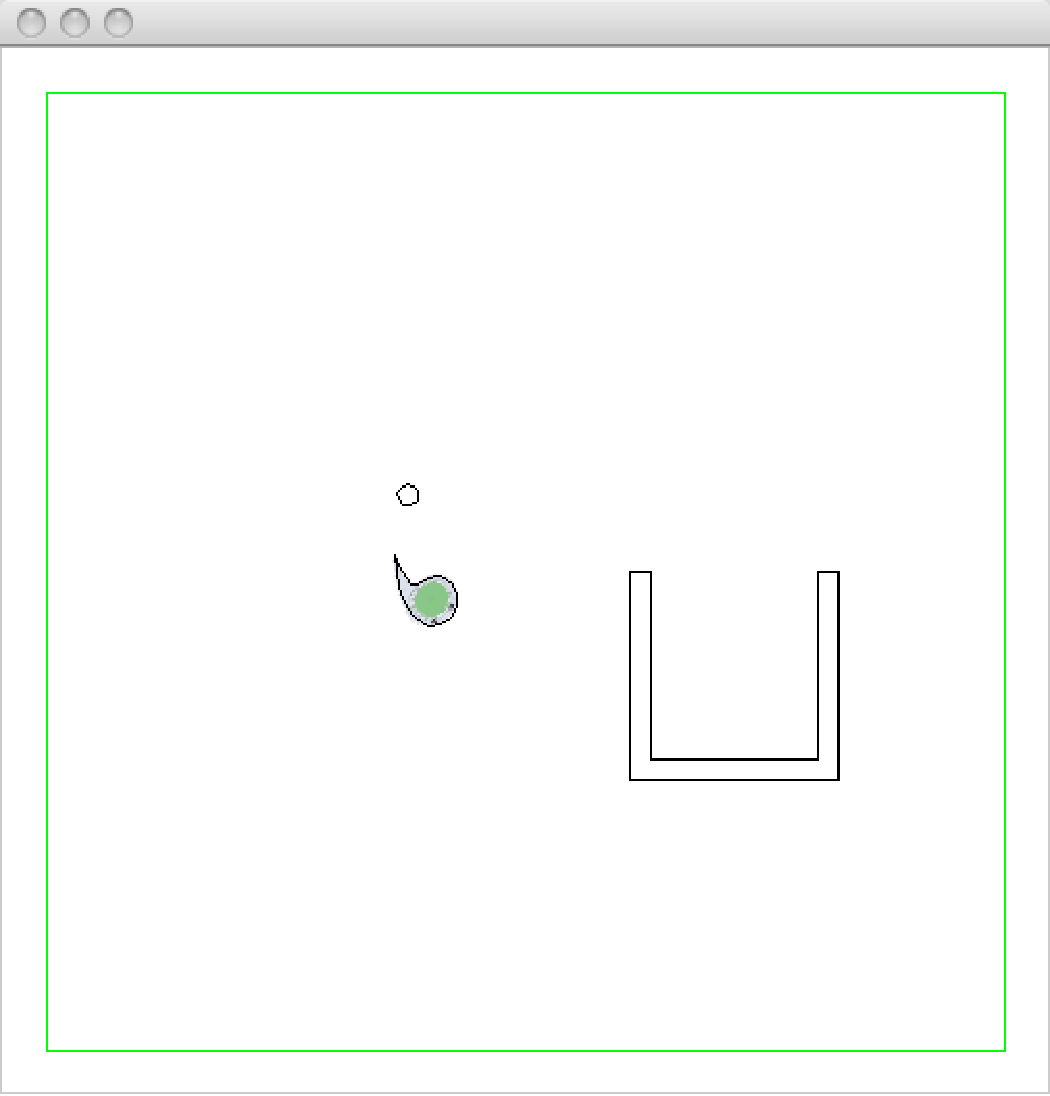
\psfig{file=images/BasketBallEnvironment.pdf,width=3in}
}
\caption{The results of using the BasketBallEnvironment class to generate 
a simulated world.}
\end{figure}

Once constructed, we can pass our environment description to the simulator
engine, which will then use it to generate a world. See \code{SimulatorMain}
for an example. Figure \ref{fig:basketball} shows the results of using the
\code{BasketBallEnvironment} class in \code{SimulatorMain}.

% @todo include BasketBall picture

\end{document}
